%! Editing first round done + spelling!
\chapter{Fock Matrix prediction}
\label{chap:fock_matrix_predictions}

SCF methods initially need a density matrix to start off their iterative calculations. Independent of the way the initial guess is chosen the computational effort of this step should be negligible compared to the actual SCF iterations.\\
As a first step we will introduce a method by which the density matrix is constructed from the Fock matrix. The later is the target for various regression and MLP models which will be introduced in the subsequent sections.


\section{Introduction}
\label{sec:Fock_mathcalrix_prediction_intro}
As explained in \autoref{subsec:background_hf_computational} the density matrix $P$ is calculated from the coefficient matrix $C$ which is obtained from the eigenvalue problem of the Fock matrix $F$:
\begin{equation}
    \label{eq:density_reconstruction_from_fock}
    F(P)\,C = SC\varepsilon \rightarrow P = 2\,\sum_{i}^{n_{occ}} C_{\mu i}\,C^*_{\nu i}\,,%2CC^T
\end{equation}
Effectively, one performs part of the SCF cycle here to obtain the density matrix, which ideally should be close to the final density matrix. This step takes $\bigO{N^3}$ time, which is asymptotically faster than $\bigO{N^4}$ time of the SCF cycles. 


\noindent
\begin{figure}[H]
    \centering
    \begin{tikzpicture}[scale=1, every node/.style={transform shape}]
        \def\imgwidth{0.30\linewidth}

        \node[anchor=south west, inner sep=0] (img1) at (0,0)
            {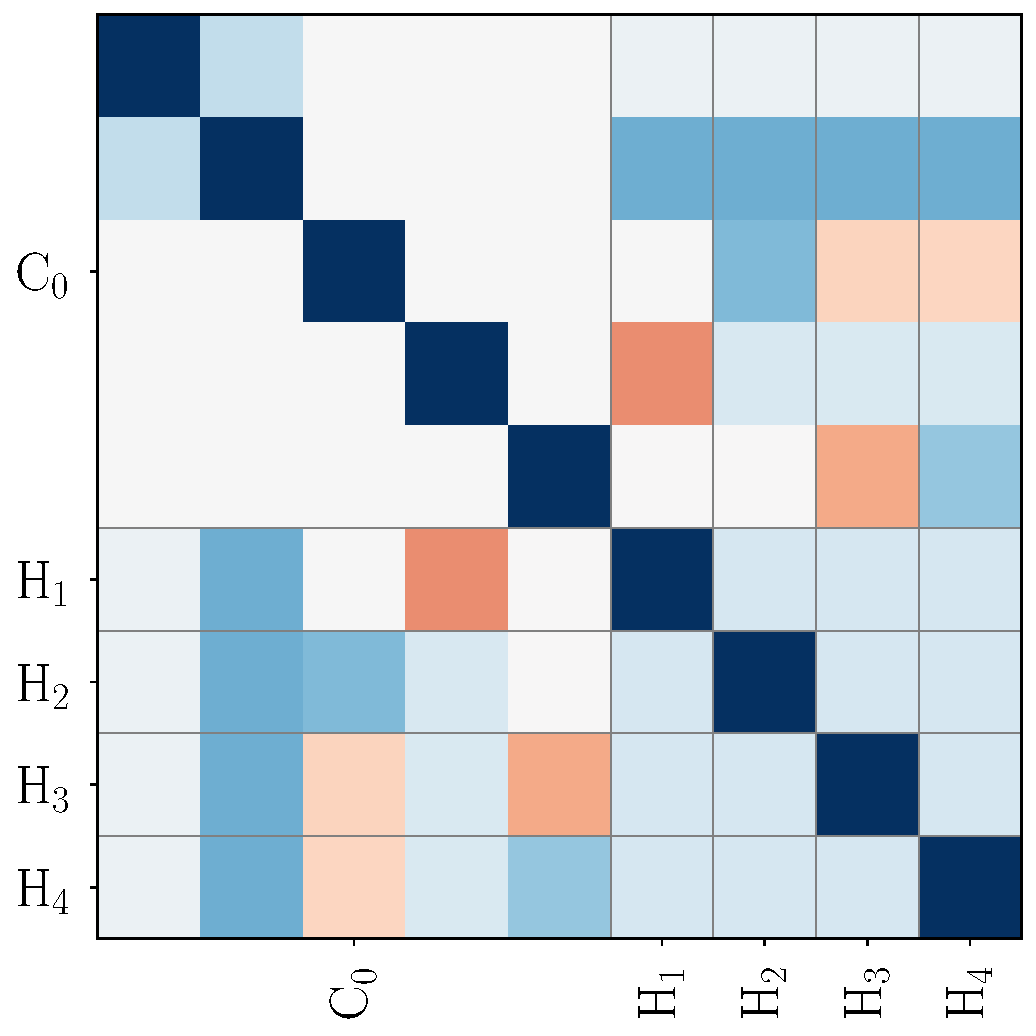
\includegraphics[width=\imgwidth]{../fig/c5h4n2o2/overlap_dsgdb9nsd_000001.pdf}};
        \node[above=2pt of img1.north, anchor=south, font=\small, xshift=10pt] {Overlap};

        \node[anchor=south west, inner sep=0] (img2) at (5.1,0)
            {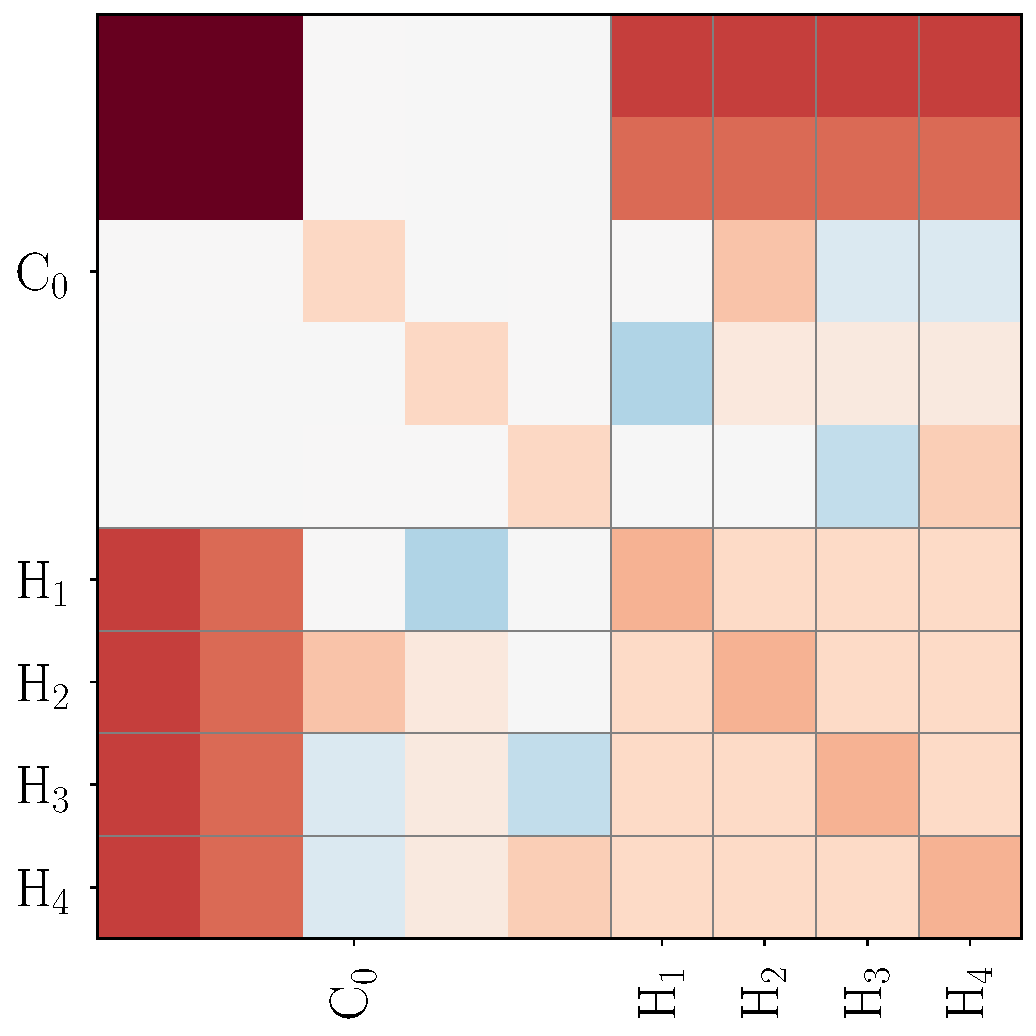
\includegraphics[width=\imgwidth]{../fig/c5h4n2o2/fock_dsgdb9nsd_000001.pdf}};
        \node[above=2pt of img2.north, anchor=south, font=\small, xshift=10pt] {Fock};

        \node[anchor=south west, inner sep=0] (img3) at (10.2,0)
            {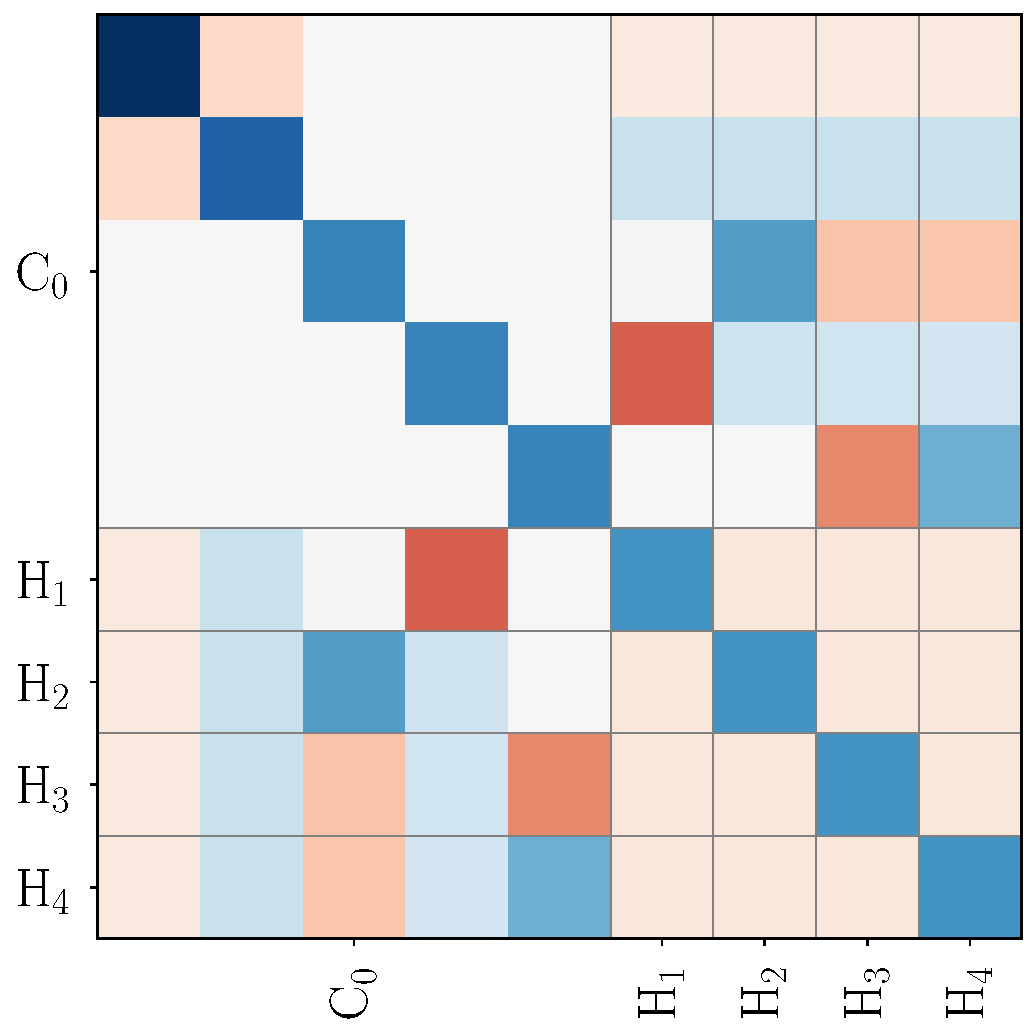
\includegraphics[width=\imgwidth]{../fig/c5h4n2o2/density_dsgdb9nsd_000001.pdf}};
        \node[above=2pt of img3.north, anchor=south, font=\small, xshift=10pt] {Density};
        
        \draw[->, thick] (4.3,2.4) -- node[above, align=center, font=\tiny]{ML\\model} (5.2,2.4);
        \draw[->, thick] (9.4,2.4) -- node[above, font=\tiny, yshift=1pt]{$P{=}2CC^{\mathrm{T}}$} (10.3,2.4);
    \end{tikzpicture}
    \caption[Schematic overview data flow]{Schematic overview of the data flow (using \ch{CH4}): overlap matrix to Fock matrix via ML model prediction, and construction of the density matrix from the Fock matrix.}
    \label{fig:method_data_flow}
\end{figure}

The schematic workflow for the generation of a density matrix from the overlap matrix is shown in \autoref{fig:method_data_flow}. Overlap and density matrices appear visually similar, which might lead to the conclusion that predicting the density matrix directly from the overlap matrix is easier. However, learning the Fock matrix tends to involve fewer strict physical constraints. A Fock matrix primarily needs to be Hermitian, while a density matrix must be strictly positive semidefinite by construction, as well as normalized to the correct number of electrons. That makes direct density matrix learning more challenging, whereas learning the Fock matrix and then obtaining the density through the diagonalisation could yield better results. We shall investigate this hypothesis in the following experiments.\\

Additionally, reconstructing the density from the Fock matrix amplifies residual errors in the predicted Fock matrix, since the density arises from a self-consistent eigenproblem involving both $F$ and $S$. Ideally, such errors should be small enough to not significantly affect the subsequent SCF iterations. In practice, some iterations (2-5) are always needed, even if one tries to run the calculation with a guessed density constructed from the converged $F$ \& $S$ matrices.\\

\section{\ch{C5H4N2O2}-subset: A first trial}
\label{sec:qm9_c5h4n2o2}

As a proof of concept we will use 508 constitutional isomers\footnote{From the 509 constitutional isomers of \ch{C5H4N2O2} 508 converged using the STO-3G basis and the B3LYP functional.} of \ch{C5H4N2O2} from the QM9 dataset. 
Single point RKS simulations in \textsc{PySCF} \parencite{ref:pyscf} were performed for these molecules using the B3LYP\footnote{B3LYPG was used to be consistent with the Gaussian program package} functional and the STO-3G basis. The resulting converged density-, fock-, and overlap-matrices were saved for future training purposes. For our very minimal basis these matrices are of size $49 \times 49$ as can be seen for a converged density in \autoref{fig:density_dsgdb9nsd_022700}. 
Due to the symmetry of the matrices we can discard nearly half of the elements and are left with 1225 features to learn. A rule of thumb for training classical statistical models is to have at least 10 samples per feature. \parencite{ref:rule_of_10} The given dataset of 508 samples is therefore far from this rule if we discard multiplicity in atoms in the samples. As a first step we shall limit our efforts to single models predicting the system based on the full overlap matrix. Nevertheless, the row / column order of our atoms in the overlap matrix has to be consistent for all the samples in the dataset (as seen in \autoref{fig:density_dsgdb9nsd_022700}). This will simply be done by sorting the atoms in the overlap matrix according to their atomic number. Now we are ready to start off our endeavour with a Ridge regression model as a first trial. 

\begin{figure}[H]
    \centering
    \includegraphics[width=\textwidth]{../fig/c5h4n2o2/density\_dsgdb9nsd\_022700.pdf}
    \caption[Density matrix of dsgdb9nsd\_022700 in the STO-3G basis with theory level B3LYP]{Converged density of dsgdb9nsd\_022700 in the STO-3G basis with theory level B3LYP. The density matrix is of size $49 \times 49$ and is symmetric. The diagonal elements in the shown AO basis correspond to Mulliken AO-populations. }
    \label{fig:density_dsgdb9nsd_022700}
\end{figure}


\section{Ridge Regressor model} % updated with new sorted dataset
\label{sec:ridge_regressor_model}
The Ridge Regressor (RR) is setup with a typical $80 / 20$ train/test split. Overlap (input) as well as Fock (output) matrices are flattened and Overlap (input) is additionally rescaled using the \textsc{scikit-learn}'s default Standard Scaler. \parencite{ref:sk-learn} Using a 5-fold cross validation the model, a Multi-Output-Regressor, is trained \footnote{also using \textsc{scikit-learn}'s \textsc{RidgeCV} and \textsc{MultiOutputRegressor} classes} with 10 equally $\log_{10}$-spaced $L^2$-regularization parameter $\alpha$ values ranging from $10^{-2}$ to $10^{3}$. Subsequently, the model is retrained with the arithmetic mean of the best performing $\alpha$ values ($\alpha_{\text{mean}} \approx 34$). This averaging reduces overfitting and yields a slightly lower RMSE on the test set compared to using individual $\alpha$ values per regressor. %! Note the averaging actually leads to a lower RMSE in test set compared to non-averaging the multi-regressor Model!  test RMSE 0.03231 vs. 0.03228 (averaging)
For the Fock matrix prediction the model yields a RMSE of $0.0057$ on the training set and $0.032$ on the test set which indicates overfitting of the model. We obtain the results in \autoref{tab:ridge_metrics} for the model and various guessing schemes implemented in \textsc{PySCF} (guessing schemes implemented in \textsc{PySCF} are listed in \autoref{sec:pyscf_initial_guessing_methods}).

\begin{table}[h]
    \centering
    \caption[\ch{C7H10O2} subset - iterations to convergence Ridge regression]{Comparison of different guessing schemes for 102 (20\%) test samples from the \ch{C5H4N2O2} subset from QM9 \parencite{ref:article1_qm9}. The average F-score is calculated on the test set using the Fock matrix prediction from the Ridge regression model and various guessing schemes implemented in \textsc{PySCF}. Furthermore averages are shown for the number of iterations until convergence and the inference time as a factor of the inference time of the \texttt{minao} guess. Not-converged reports the percentage of samples not converging within 50 iterations.}
    \label{tab:ridge_metrics}
    \resizebox{\textwidth}{!}{
    \begin{tabular}{l
                    S[table-format=1.2(2)]
                    S[table-format=1.3(3)]
                    S[table-format=1.2(2)]
                    S[table-format=1.3(3)]
                    S[table-format=1.3(3)]
                    S[table-format=1.3(3)]}
        \toprule
        \textbf{Method} & \texttt{Ridge-model} & \texttt{minao} & \texttt{1e} & \texttt{atom} & \texttt{hückel} & \texttt{vsap} \\
        \midrule
        F-score / 1 & 0.93 \pm 0.04 & 0.899 \pm 0.002 & 0.71 \pm 0.02 & 0.802 \pm 0.0010 & 0.840 \pm 0.010 & 0.993 \pm 0.002 \\
        Iterations / 1 & 14 \pm 3 & 11.7 \pm 1.0 & 23 \pm 4 & 11.4 \pm 0.8 & 22 \pm 6 & 12.8 \pm 1.1 \\
        Inference-speed / 1 & 0.7 \pm 0.3 & 1.0 &  0.05 \pm 0.02 & 0.5 \pm 0.4 & 0.5 \pm 0.3 & 3 \pm 1.3 \\
        Not-Converged / \% & 4 & 0 &  31 & 0 & 27 & 0\\
        \bottomrule
    \end{tabular}
    }
\end{table}
Ridge regression performs better than the \texttt{1e} and \texttt{hückel} guessing schemes in terms of iterations but still fares worse in comparison to the \texttt{minao}, \texttt{atom} and \texttt{vsap} guessing schemes. It should be noted that there seems to be no significant correlation of the F-score with the number of iterations till convergence. While \texttt{vsap} yields by far the highest F-score, it on average takes one iteration more to converge than the \texttt{minao} guessing scheme. This hints at the fact that some guessing strategies might guess better in regions in the density matrix which are more relevant for convergence speed than others. \\
Comparing the normalized difference to the reference density for the 102 test sample for \texttt{minao}, \texttt{vsap} and the Ridge regression model in \autoref{fig:density_error_comparison} gives different error patterns.  

\begin{figure}[H]
    \centering
    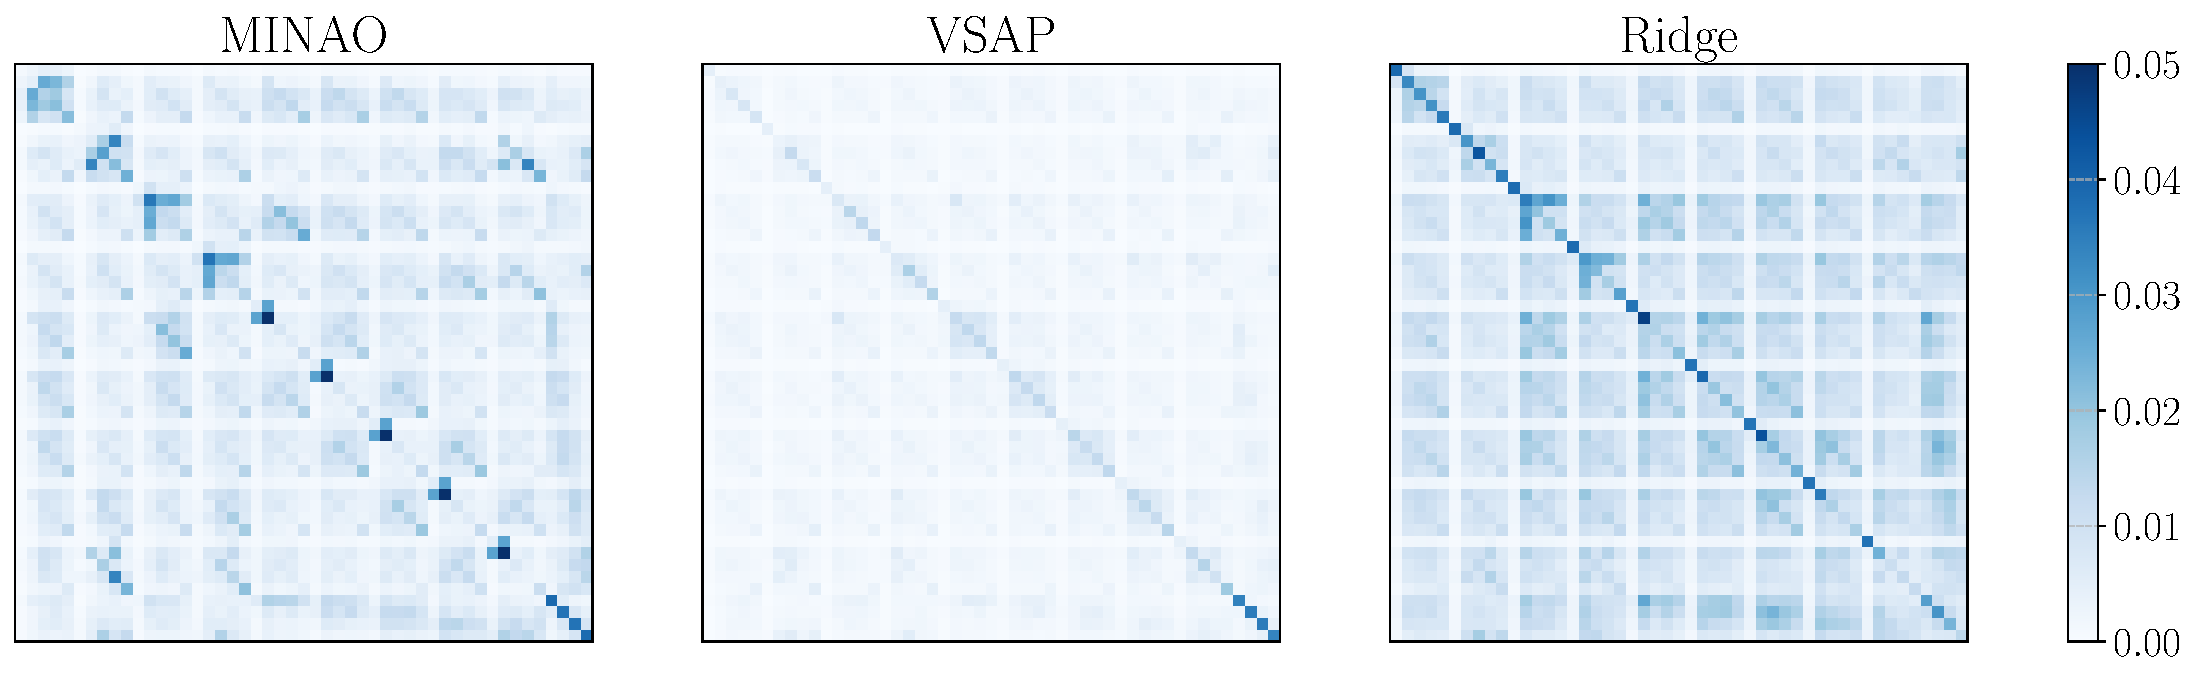
\includegraphics[width=\textwidth]{../fig/c5h4n2o2/density_error_comparison.pdf}
    \caption[Normalized difference of density guesses]{Normalized mean absolute difference of $\alpha$-electron density guesses to their converged density for \texttt{minao} \& \texttt{vsap} guess and the Ridge regression model evaluated on the test set: 102 (20\%) test samples from the \ch{C5H4N2O2} subset from QM9 \parencite{ref:article1_qm9}.}
    \label{fig:density_error_comparison}
\end{figure}
All three guessing schemes have spots on the main diagonal of the density matrix where they are likely to differ from the reference solution. Interestingly, a Mulliken population analysis (see \autoref{subsec:background_hf_derived_quantities}) \parencite{ref:Mulliken_population_analysis} yields a mean value of $31.766$ on the test set prediction for \texttt{minao} while \texttt{vsap} yields the expected $32$ (only $\alpha$-electrons). A small error in the initial guess doesn't slow down convergence, since the self-consistent cycle corrects it right away. Comparing \texttt{minao} and \texttt{vsap} with our Ridge Model the later fares worse on the main diagonal, especially for p-Orbitals. While \texttt{minao} exhibits more pronounced off-diagonal noise in comparison to \texttt{vsap}, this does not seem to affect convergence speed. At least for this small basis set, errors in the off-diagonal elements do not appear to hinder fast convergence.\\
% From that we might conclude that a good guess should be close to the reference density especially on the main diagonal, but not necessarily in the off-diagonal elements. We shall continue to investigate this in the next section.

\section{Kernel Ridge Regression}
\label{sec:kernel_ridge_regression}
Our baseline Ridge Regression (RR) model already introduced $L^2$-regularization handling collinearity which is doomed to happen in our dataset. However, it only models linear relationships between our input and output features. Kernel Ridge Regression (KRR) extends this by using kernel functions to generate a mapping from the input space via a higher dimensional feature space to the output space. This allows nonlinear relationships to be learned. \\
Using the same train/test split as before we fit a KRR model with three different kernels: RBF, polynomial of degree 2 and polynomial of degree 3. 
Rather than averaging per-target $\alpha$ values (like in the RidgeCV above), we use a joint BayesSearch with 5-fold cross validation and 30 iterations\footnote{Hyperparameters see \autoref{tab:kernel_ridge_hyperparams}} to obtain the results in \autoref{tab:kernel_ridge_metrics}.

\begin{table}[h]
    \centering
    \caption[\ch{C7H10O2} subset - iterations to convergence Kernel Ridge regression]{Comparison of different Kernel Ridge regression (KRR) guessing schemes for 102 (20\%) test samples from the \ch{C5H4N2O2} subset from QM9 \parencite{ref:article1_qm9}. The F-score is calculated using the Fock matrix prediction from the Kernel-Ridge regression model and the \texttt{minao} guess. The number of iterations until convergence is shown as well as the percentage samples not converging within 50 iterations and the inference time as a factor of the inference time of the \texttt{minao} guess.}
    \label{tab:kernel_ridge_metrics}
    \resizebox{\textwidth}{!}{
        \begin{tabular}{l
                        S[table-format=1.2(2)]
                        S[table-format=1.3(3)]
                        S[table-format=1.2(2)]
                        S[table-format=1.3(3)]}
            \toprule
            \textbf{Method} & \texttt{KRR RBF} & \texttt{KRR quadratic poly} & \texttt{KRR cubic poly} & \texttt{minao} \\
            \midrule
            F-score / 1         & 94 \pm 4 & 94 \pm 4 & 53 \pm 1.5 & 0.899 \pm 0.002 \\
            Iterations / 1      & 14 \pm 3 & 14 \pm 3 & 20 \pm 5 & 11.7 \pm 1.0 \\
            Inference-speed / 1 & 30 & 20 & 19 & 1.0\\ %! This is obviously very amusing in terms of uncertainty (therefore no uncertainty here)
            Not-Converged / \%  & 4 & 4 & 12 & 0\\
            \bottomrule
        \end{tabular}
    }
\end{table}
Hyperparameters found by the BayesSearch are shown bellow in \autoref{tab:kernel_ridge_hyperparams}.

\begin{table}[h]
        \centering
    \caption[Hyperparameter Kernel Ridge regression]{Hyperparameters found using BayesSearch for the Kernel Ridge regression models with different kernels.\\Search space: $\alpha \sim \operatorname{LogUniform}(10^{-8},10^{4})$, $\gamma \sim \operatorname{LogUniform}(10^{-6},10^{3})$ and $\mathrm{coef0} \sim \operatorname{Uniform}(0,1)$ for polynomial kernels; for the RBF kernel $\mathrm{coef0}$ is ignored}
    \label{tab:kernel_ridge_hyperparams}
    \begin{tabular}{l
                    S[table-format=1.0e1]
                    S[table-format=1.1e1]
                    S[table-format=1.1e1]}
        \toprule
        \textbf{Hyperparameter} & \texttt{KRR RBF} & \texttt{KRR quadratic poly} & \texttt{KRR cubic poly}\\
        \midrule
        $\alpha$ & 2e-8 & 1e-8 & 5e-2 \\
        $\gamma$ & 4e-5 & 7e-5 & 1e-6 \\
        $\mathrm{coef0}$ & \text{-} & 7.5e-1 & 1.4e-1 \\
        \bottomrule
    \end{tabular}
\end{table}

While RBF and quadratic kernels yield nearly comparable results, with the exception of inference speed, the cubic kernel performs significantly worse. The underperformance of the cubic kernel is to be explained by the fact that the Bayes search gave a relatively high $\alpha$ value of $0.05$ which leads to a strong regularization of the model making it less flexible. Even with lower regularization the cubic kernel, as well as the other two kernels, does not yield comparable performance to the \texttt{minao} guessing scheme. Interestingly, our models yield a significantly higher F-score (exception: cubic kernel) compared to \texttt{minao} but take more iterations to converge. A pattern which we have seen before with the Ridge regression model emerges again. This and the inefficient scaling of KRR with the number of samples leads us to explore different approaches in the next section.\\ 



\section{Further trials using MLP}
\label{sec:further_trials_mlp}
Previously, we tried to learn a mapping from overlap to Fock matrix solely via machine learning means. We have established that the quality for these guesses even on the minimal STO-3G basis is not on par with the established guessing schemes.\\
Predicting the main diagonal for a given system is an easier target given the fact that the model predicts $N$ features from the $N^2$ input features. One established way of constructing the off diagonal elements is the generalized Wolfsberg-Helmholtz (GWH) construction \parencite{ref:gwh_wolfsberg1952spectra} (see \autoref{eq:gwh}).
Utilizing this construction on our dataset we obtain comparable results to our base Ridge regression model in terms of iterations till convergence. \\
Changing the basis set to a larger 6-31G(2df,p) one, we see the limitations of our initial approach. Instead of roughly $\nicefrac{49^2}{2}$ features we now have $\nicefrac{254^2}{2}$, a nearly 27-fold increase in the number of features. Furthermore, we will move to an isomer offering more samples for training, namely the 6095 \ch{C7H10O2} structural isomers (this set of isomers will also be used to benchmark the GNNs in \autoref{chap:gnn}).\\

\textbf{MLP Network}\\
We implement a MLP model which is trained to map the overlap matrix to the main diagonal of the converged Fock matrix from which density can be reconstructed via GWH. All samples are split into 80\% training, 10\% validation and 10\% test sets. Batch wise data loading was implemented to facilitate training on memory limited hardware. To gauge the performance of different configurations a hyperparameter search was performed over the parameters in \autoref{tab:hyperparams_mlp}.

\begin{table}[h]
    \caption[Hyperparameter \& Parameters of the MLP model]{Hyperparameter \& Parameters of the MLP model. Model with best parameters marked bold.}
    \label{tab:hyperparams_mlp}
    \centering
    \begin{tabular}{@{}ll@{}}
        \toprule
        \textbf{Hyperparameter}     & \textbf{Search Space}                  \\ 
        \midrule
        \texttt{layers / 1}          & $\{\textbf{1},\,2,\,3,\,4\}$                         \\
        \texttt{neurons / 1}   & $\{256,\,512,\,\textbf{1024}\}$  separate for each layer    \\
        \texttt{dropout rate / \%}   & $\{0,\,5,\,\textbf{10},\,15,\,20\}$ separate for each layer \\
        \bottomrule
        \textbf{Parameters}     & \textbf{Value}                  \\ 
        \midrule
        \texttt{layer type}          & dense                         \\
        \texttt{activation}          & gelu                         \\
        \texttt{batch normalization} & after each hidden dense layer \\
        \texttt{batch size}          & 32 \\
        \texttt{input dimension}     & 40470 \\
        \texttt{output dimension}    & 284 \\
        \bottomrule
    \end{tabular}
\end{table}

\texttt{Tensorflow} was used as backend with \texttt{Keras} and the module \texttt{Keras\_tuner} for hyperparameter optimization. \parencite{ref:tensorflow,ref:keras,ref:kerastuner}
All models in the hyperparameter optimization where trained using the Adam optimizer with an exponential decay (rate $0.96$ every 100 batches). Using mean squared error as the optimization objective on the validation set, Hyperband tuner selected a single-layer MLP with 1024 neurons and a 10\% dropout rate.\\
Subsequently, this model was retrained for 50 epochs for initial evaluation on the test set. A prediction performance (RMSE on test set) of $\num{0.1 \pm 0.014}$ compared to $\num{0.357 \pm 0.007}$ \texttt{minao}'s on the main diagonal looks promising. However, after reconstructing the full Fock matrix using \autoref{eq:gwh} the global prediction quality on the full matrix suffers drastically as seen in \autoref{fig:comparison_mlp_gwh_fock}. 

\begin{figure}[H]
    \centering
    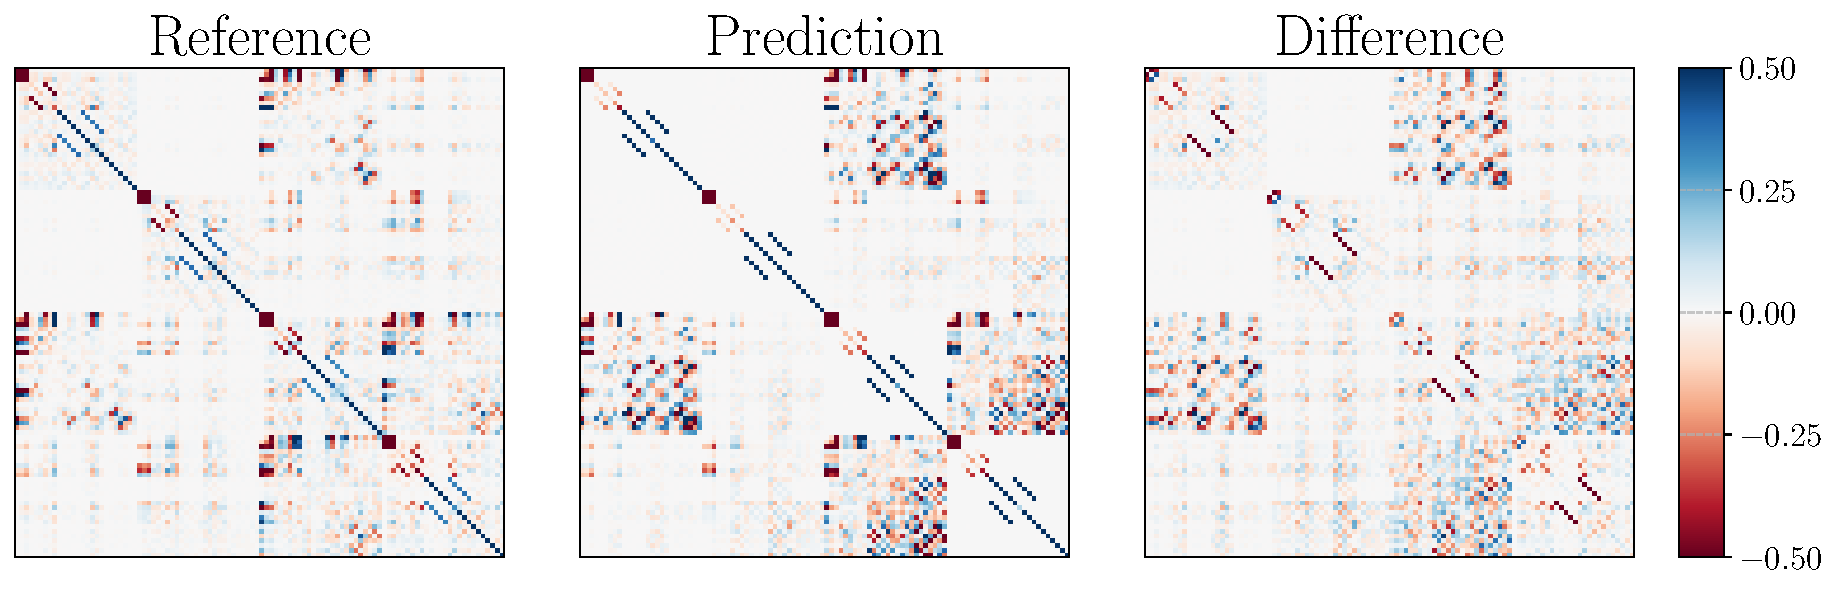
\includegraphics[width=\textwidth]{../fig/mlp_further_trials/fock_truth_vs_pred.pdf}
    \caption[MLP vs. reference Fock]{Reference (fully converged Fock matrix) vs. predicted Fock matrix using the MLP model and the GWH re-construction and element-wise difference for \texttt{dsgdb9nsd\_082452}. Plots only show entries for two \ch{O} (upper left) and two \ch{C} (lower right) atoms and their respective off-diagonal elements.}
    \label{fig:comparison_mlp_gwh_fock}
\end{figure}

\begin{figure}[H]
    \centering
    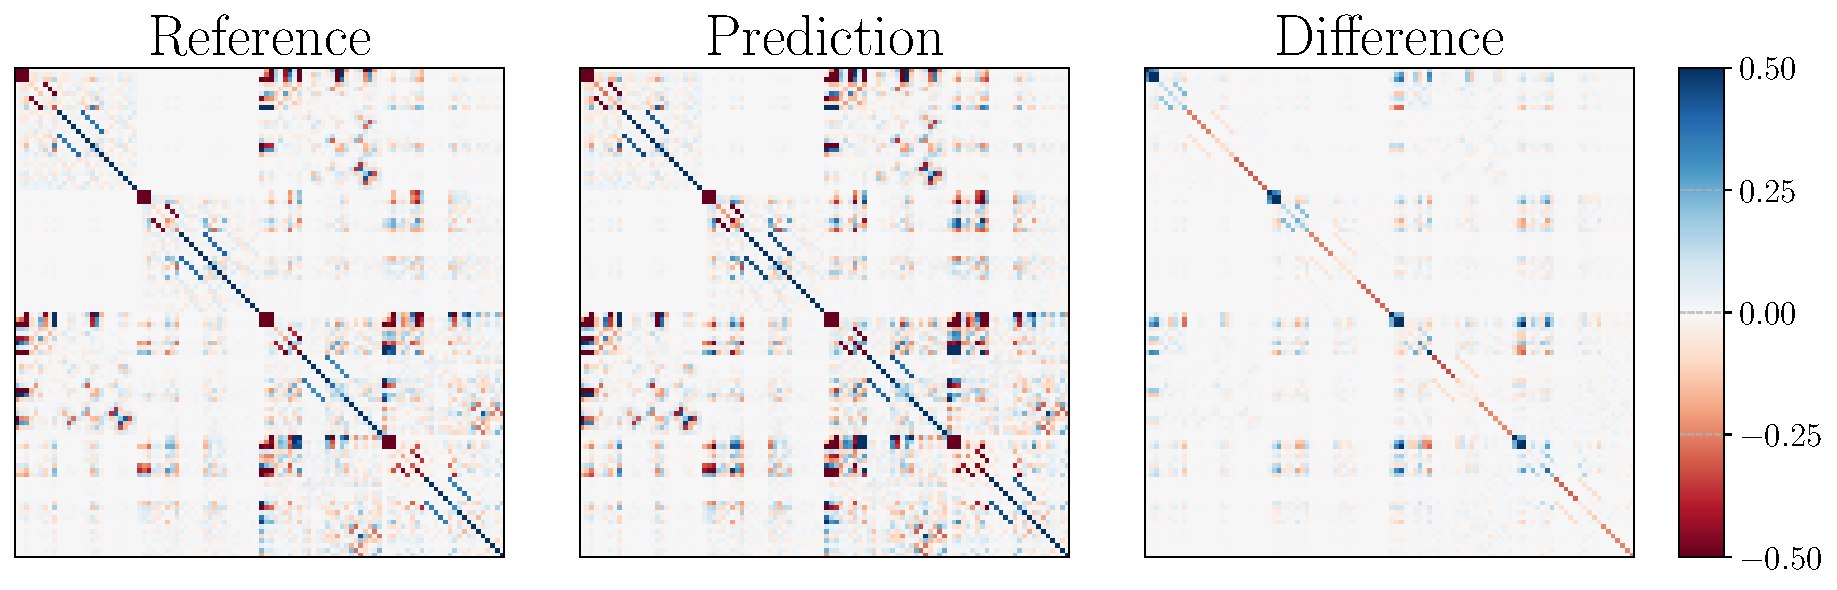
\includegraphics[width=\textwidth]{../fig/mlp_further_trials/fock_truth_vs_minao.pdf}
    \caption[\texttt{minao} vs. reference Fock]{Reference (fully converged Fock matrix) vs. Fock matrix constructed via \texttt{minao} guess and element-wise difference for \texttt{dsgdb9nsd\_082452}. Plots only show entries for two \ch{O} (upper left) and two \ch{C} (lower right) atoms and their respective off-diagonal elements.}
    \label{fig:comparison_minao_fock}
\end{figure}
Comparing \autoref{fig:comparison_mlp_gwh_fock} and \autoref{fig:comparison_minao_fock} the difference in error patterns is apparent. While the MLP model performs well on the main diagonal, the GWH reconstruction cannot adequately capture the off-diagonal elements, thus resulting in a high RMSE of $0.085$ compared to $0.029$ for the \texttt{minao} guess. Given that many entries are zero—thereby artificially lowering the overall RMSE—the roughly three-fold difference further highlights the substantial underperformance of the GWH reconstruction compared to the \texttt{minao} guess.\\
To get the density from our Fock matrices we solve \autoref{eq:density_reconstruction_from_fock} and gather the lowest $n_{occ}$ eigenvectors to build the coefficients and subsequently the density matrix. The density obtained by this procedure is shown in \autoref{fig:comparison_mlp_gwh_density} and compared to the density obtained from the \texttt{minao} guess directly.

\begin{figure}[H]
    \centering
    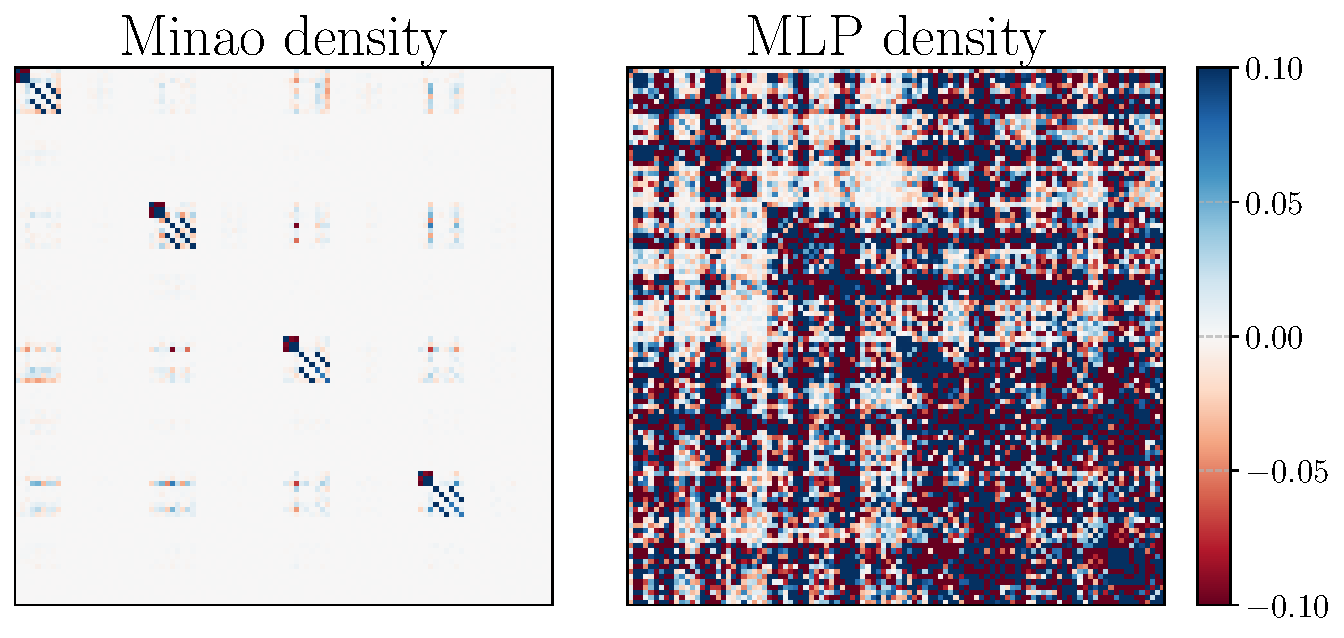
\includegraphics[width=0.7\textwidth]{../fig/mlp_further_trials/minao_vs_pred.pdf}
    \caption[\texttt{minao} vs. MLP density]{\texttt{minao} density vs. density given by the diagonalisation of the Fock prediction from the MLP model for \texttt{dsgdb9nsd\_082452}. Plots only show entries for two \ch{O} (upper left) and two \ch{C} (lower right) atoms and their respective off-diagonal elements.}
    \label{fig:comparison_mlp_gwh_density}
\end{figure}
While \texttt{minao} provides a sparse density matrix, our MLP implementation yields a very dense result with many non-zero-off-diagonal elements. This directly stems from the fact that GWH does introduce large errors in the Fock matrix which propagate through the eigenvalue problem to the density matrix. \\
A qualitative benchmark of iteration count till convergence offers a similar picture as before: Calculations using the \texttt{minao} guess converge in roughly 11 iterations, while the simulations using the MLP model with GWH reconstruction take around 20 iterations. The present model thus performs similar to other basic initialization schemes such as the \texttt{1e} guess. Interestingly, our model and the \texttt{1e} guess do not offer statistically relevant benefits in terms of iterations compared to a randomly initialized density matrix as seen in \autoref{tab:mlp_metrics}.
\begin{table}[h]
    \centering
    \caption[\ch{C7H10O2} subset - iterations to convergence MLP]{Iterations needed to convergence for different guessing schemes on the \ch{C7H10O2} test subset. MLP\_GWH uses the MLP prediction with GWH reconstruction of Fock off-diagonals and subsequent derivation of density matrix. The \texttt{random} column refers to a random density guess in the range $[-0.5, 0.5]$}
    \label{tab:mlp_metrics}
    \begin{tabular}{l
                    S[table-format=2.1(1)]
                    S[table-format=2(1)]
                    S[table-format=2.1(1.1)]
                    S[table-format=2.1(1.1)]}
        \toprule
        Method          & {minao} &{1e}& {MLP\_GWH}        & {random}  \\
        \midrule
        Iterations (\#) & 10.8(4) & 19(3)  & 19.8(1.0) & 19.8(1.2)       \\
        \bottomrule
    \end{tabular}
\end{table}

\section{Conclusion}
\label{sec:fock_matrix_prediction_conclusion}
This chapter introduced an approach to predict the density matrix by first estimating the Fock matrix and then reconstructing the density via diagonalisation. Initial experiments on the \ch{C5H4N2O2} subset of QM9 showed that linear models (Ridge Regression and Kernel Ridge Regression) can learn the Fock matrix reasonably well but fail to match the accuracy of established PySCF guessing schemes such as \texttt{minao} and \texttt{vsap} in terms of iterations till convergence. When scaling up to a larger 6-31G(2df,p) basis and the \ch{C7H10O2} isomer set, a single-layer MLP captured the Fock diagonal with low RMSE, yet the generalized Wolfsberg-Helmholtz reconstruction of off-diagonals introduced large errors. Diagonalisation amplifies these errors, producing a noisy density matrix and nearly doubling SCF iterations ($\approx20$ vs. 11).

Overall, while the ML-based Fock prediction pipeline can outperform simple Hückel or one-electron guesses in diagonal accuracy, it still underperforms in convergence speed and off-diagonal fidelity compared to better physics-based schemes. This suggests that a one-shot prediction of the full Fock matrix simultaneously ans subsequent density derivation is infeasible. Accounting for local interactions and directly predicting a sparse density matrix (compared to the Fock matrix) may perform  better. We shall explore the later approach in the next chapter by representing molecular structure using a Graph Neural Network (GNN). 

